\chapter{The Neutral apparatus}
\label{ch:chap2}

Our experiments begin by cooling and trapping atomic strontium utilizing well-established atomic physics techniques \cite{Metcalf1999,Katori1999,Ido2000,Nagel2003,Mukaiyama2003a,Loftus2004,DeEscobar2009a,Stellmer2009,Stellmer2010,Mickelson2010,DeSalvo2010,Tey2010a}. Fig.\;\ref{fig:energy_level_diagram} shows the simplified energy level diagram employed in our cooling process. Once cooled, we typically obtain bulk samples in an optical dipole trap containing on the order of $10^6$ atoms at temperatures $<1\mu$K and densities between $10^{12} - 10^{15}\,$cm$^{-3}$ depending upon the isotope. Samples of ultracold atoms can then be directly loaded into an optical lattice potential by ramping up the intensity of the laser beams forming the optical lattice.


Brians thesis
refs - [27, 28, 29, 30, 31, 32] for cooling and trapping

The Neutral apparatus was one of the pioneering experiments for the trapping, cooling, and creation of quantum degenerate gases of neutral strontium. As such, there is a plethora of previous theses and publications which extensively outline the details for how to achieve these goals. \hl{refs}. In particular, we refer the reader to the PhD theses of previous Killian lab students, Brian DeSalvo, Mi Yan, Pascal Mickelson, Natali Martinez de Escobar, and Sarah Nagel.

Building upon this previous work, this chapter will forego an extensive review of the basic laser cooling techniques for strontium. Instead, we will briefly discuss the systems and processes which are most crucial to the operation of the experiment with an emphasis on technical findings and changes which remain, as of yet mostly, undocumented.

This chapter is meant to serve as a highly technical and in-depth guide to the operation of the Neutral apparatus. We refer the reading to the extensive works for a discussion of the theory behind laser cooling and trapping.

\section{Experimental Procedure} \label{sec:trapping}
This section will 

\section{Vacuum system and atom source}
\label{sec:vac}

Diagram
Description
	very good resource for design considerations of a similar experiment in Francy's masters chapter 3
	Appendix A.10 of Natali's thesis gives specifics about the construction
Components
	Atom Source
	2D collimator
	Zeeman slower
	main chamber
	Cryo tower
History
	

	
Zeeman slower
	constructed by Pascal
	


Details of the consturction of the vaccuum system are available in \hl{so and so}

The goal of this section is to provide an overview of the most recent history of the vaccuum system as well as to clarify some of the slightly more ambiguous points about what the construction of the apparatus.

Potentially discuss the concerns we've had about the platform and movement between the chamber and the table. THis can lead to the addition of struts tying the chamber to the platform. This remains a source of concern for heating of the atoms particularly in the optical lattice. 

These concerns are exacerbated by an our finding that increased stability came when adding a partial cover over the platform optics for the optical dipole and lattice traps. Although initially meant as a proctective measure, the addition of this cover resulted in a noticable decrease in shot to shot fluctuations of the cloud position after a time of flight. We found that this stability was a result of mitigating air currents due to the closely located ventilaition system meant to mitigate dust acculation on the optical components.

Drawings for the atom source currently in use on the experiment (as of March 2019) are available in the App \hl{vaccuum}. This oven design is labeled "new nozzle summer 2010", and outlines a heat shield that was ultimately abandoned due to lack of a mechanism to secure it to the base flange. This led to the heat shield falling off when attempting to secure the flange in the apparatus. We hypothesized that lack of a heat shield led to uneven distribution of the thermal energy throughout the oven so we undertook the design of a new oven design to address this issue.

The Neutral apparatus is built around a stainless steel chamber positioned so and so above the table to facilitate optical access as described \hl{somewhere}. While unchanging during the time of this phd we have learned a number of crucial 

Pressuess within this chamber ar typically of the order blah

The system consists of an oven source based around a custom nozzle design
Starting from left to right we have a 6 way tee as the main body for the atom source, a 2D coliamtor, and the entry port of the 1 meter zeeman slower. Somewhere in here is a connection to an ion pump.
There is a differential pumping tube annd needles on he atom source. Throught he zeeman slower we connect to the main chamber which is a custom 304 stainless steel body supported by a pumping tower which is the entry point for the zeeman laser beam and an additional ion pump. 

In the late fall of 2017 the neutral apparatus had been under vaccuum for approx 6? years and ater extensive testing we determined that we likely ran out of elemental strontium within the atomic source. This led us to breaking vaccuum, reloading strontium, and performing a small bake down procedure to restablish our presssure. ripor to this event we enjoyed lifetimes on the ordr of 25s s measured by background lifetimes measurements within our IR optical dipole trap. Apprximately a year affter this event we have observed lifetimes on the order of approx 15s, the cause of the discrepanacy is currently unknown.
During the time of breaking vaccuum we decided to attempt everal upgrades to the apparatus such as adding a gate valve between the pumping tower and the zeeman window and redesigning the nozzle source to incorporate a heat shield around the heating element to produce a more even heating environemnt along the nozzle
De to timing we did not install the gate valve before re-establishing vaccuum. The hope in doing this upgrade was to provide a better method for replacing the end cap window which the atom source directly points at. During the course of our experiments this window slowly accumulates a thin layer of strontium which may act as a parital mirror and attentuate the crucially important zeeman beam. As a note of interest, it was shared through private communication with professor Killain that pulsed 532 nm light (such as from a q-locked Verdi system used in the Plasma laboratory) might vaporize the strontium off the window and restore any loss in power. Using a test appartus we were able to verify that indeed we can ablate the strontium off of a coated window, as shown in figure something.
This promising test led us to install an optical traversal port, shown in figure, connecting the two labs. Unfortunately, while flashing the verdi on a small section of the neutral experimental window we found that the energy needed to ablate the strontium was accompanied by deformation of the optical surface of the window. We attritbute this to the thicknes of the coating as the key difference between the experiment and the Neutral machine.
With that fun aside, we oder an extra window and the gate valve to replicate the system put in place on the Rydberg appartus so that future needs to repalce the window coul be accomplished by simply back filling the chamber with dry nitrogen or argon, closing the gate valve and simply replacing it quickly without the need to expose the main chamber body to direct atmospheric gas. 

Reudction of the time the window was exposed to hot strontium led us to install a small servo motor driving the valve (model something) and integrate this mechanism into the experimental runtime. This allows the shutter to only be open during the times that we are actively trapping atoms. Details of the servo motor trigger integration into the neuKLEIN control system are available in App \hl{somewhere}.

The second improvement that we attempted was to redesign the nozzle to include a heat shield. A CAD image is shown in figure. Unfortunately, due to the high tolerances of the base flange and surrounding enclosure the machining required for this custom piece was deemed prohibitvely expensive. A prototype was design following the machine drawings available in App \hl{someplace} but was abandoned due to a bend that developed in the tubing which holds the fire rod. 

However, the largest constraint was due to the flange size of 2 3/8" as the basis for the design. This provides very tight confinement and w

What is the model number for the firerod? What were the materials that were used? 

During the course of realignment of having the vaccuum chamber open, we took the opporuntity to replace the atom source with an uncoated window to aid alignment of the zeeman beam through the entire length of the vaccuum system. While doig this we learned that there is a slight angle to the differential pumping tube which separates the atom source chamber from 2D collimation chamber. While we were not able to determine the severity of the misalignment the main symptom of its existence is the partial occlusion and loss of power in the zeeman slowing beam. With an input power of approx. 120 mW before expansion optics and entering the chamber, we measured 60 mW of power transmitted through the window during our testing. Replacement of this differential pumping tube is problematic as it is part of a copper flange held between flanges connecting the aomt source chamber and 2D collimator. This positioning necessitates a drastic and practically infeasible deconstruction of the vaccuum system to replace. Our goal here is simply to inform future students of this issue as we believe it is the primary cause of the much longer load times needed in the Neutral apparatus when compared to the newly designed Rydberg machine.


	\begin{figure}
		\centerline{
		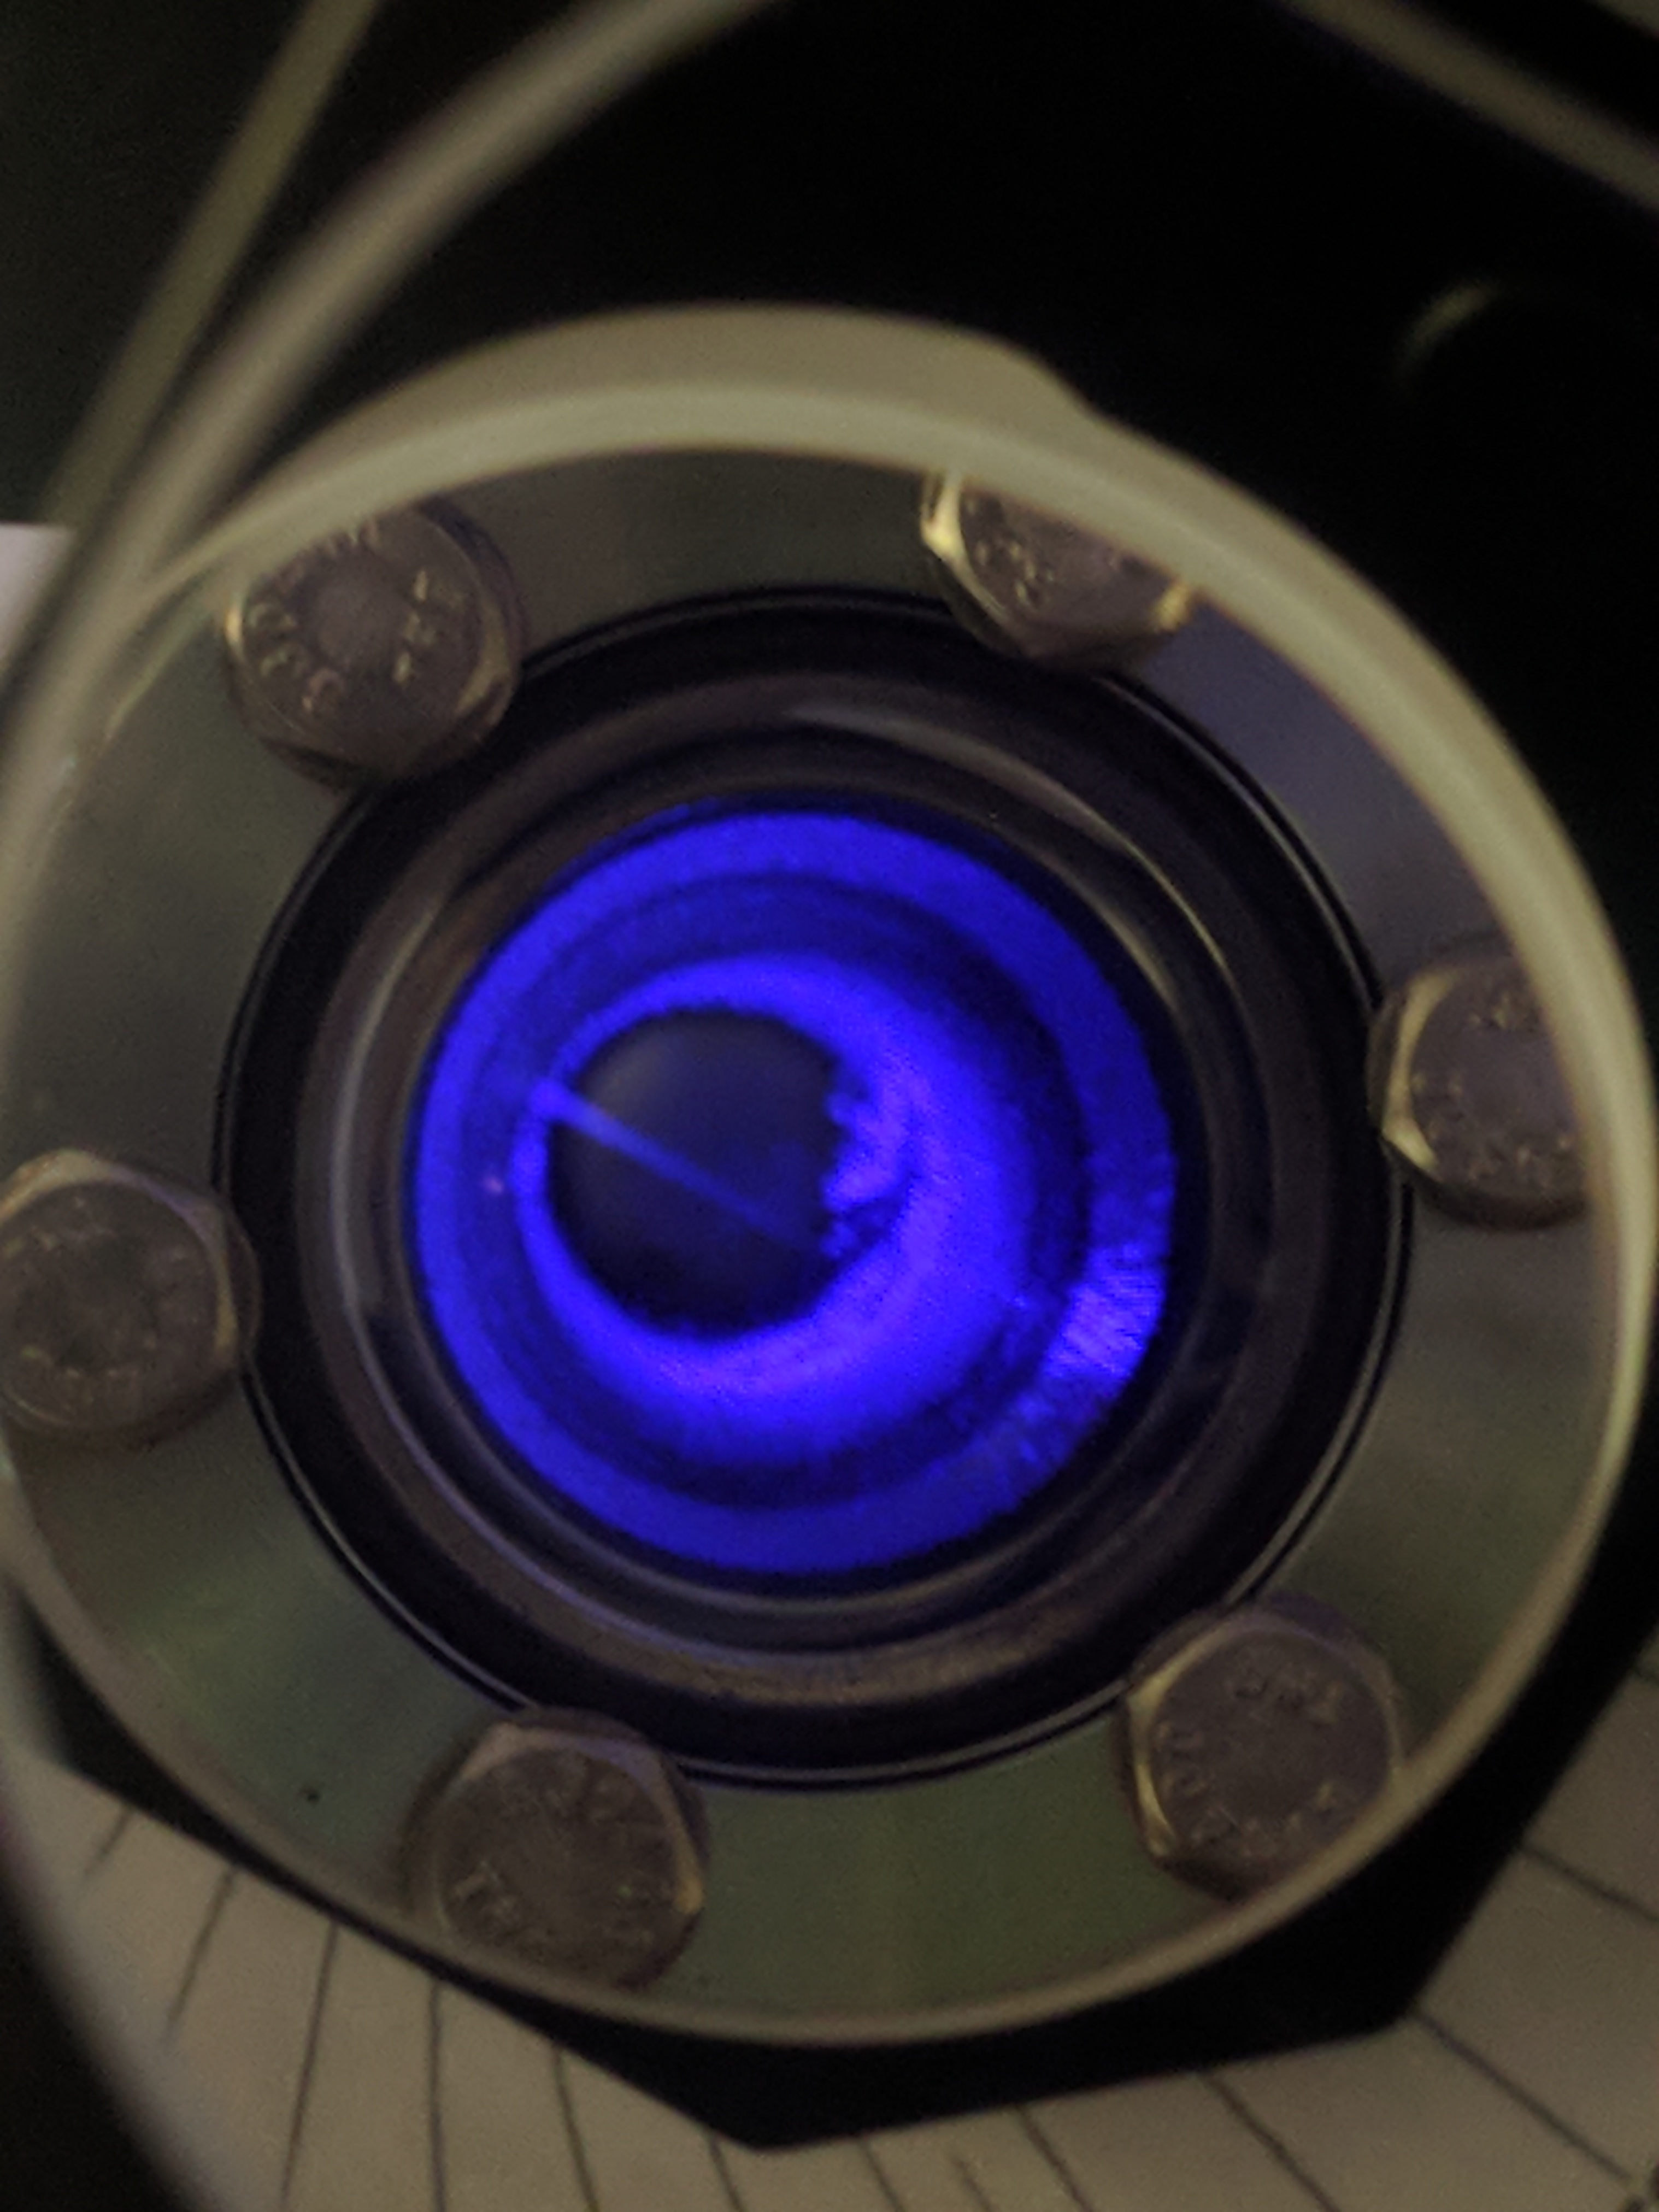
\includegraphics[width=\textwidth]{IMG_20171103_184230.jpg}}
		\caption{Typical flourescence of Zeeman beam looking down 2D collimator}{This view is found using a 2 in mirror aligned along the path of the first pass of the 2D collimator (near mirror 3 in the diagram), looking down the collimator tube. While looking at this angle, we are able to see the Zeeman beam move across the atom column when moving the last turning mirror. Reduction in this fluorescence signal from that shown was the primary indicator of lack of strontium in the source.}
		\label{fig:2d_coll_flourescence}
	\end{figure} 
	
	\begin{figure}
		\centerline{
		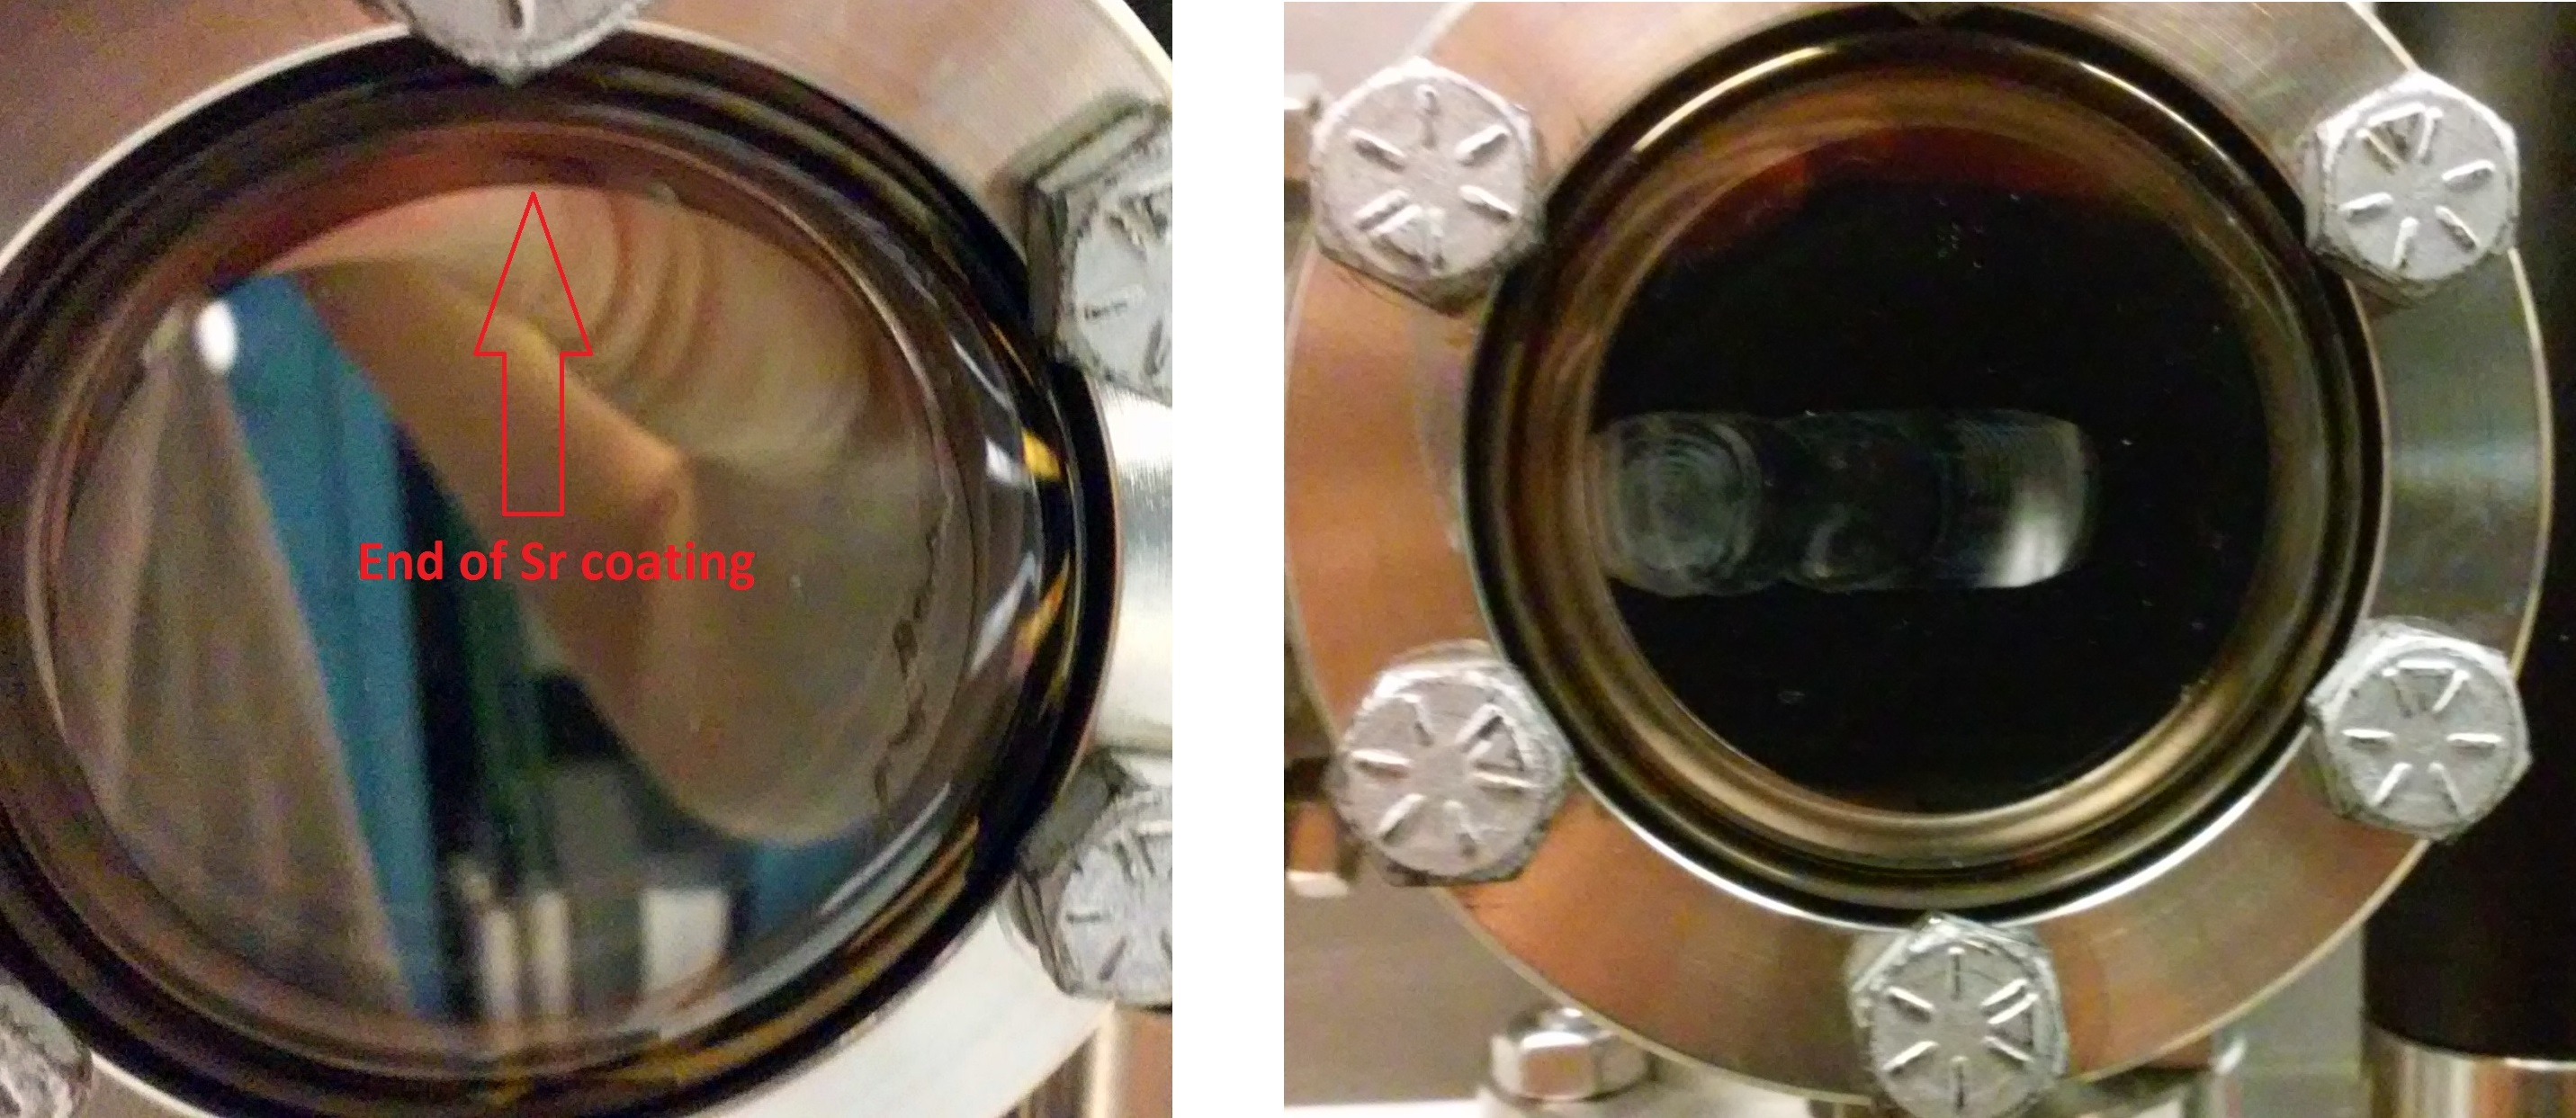
\includegraphics[width=\textwidth]{ablated_sr2.jpg}}
		\caption{Ablating strontium coating from window}{Comparison of the before (left) and after (right) when using a pulsed 532 nm Verdi to ablate strontium. The residue visible in the after image was due to a higher energy pulse which was reduced as we moved towards the center of the window.}
		\label{fig:ablating_strontium}
	\end{figure} 



\section{Laser systems}
\label{sec:laser_systems}

The heart of any atomic physics experiment is the laser systems which can be utilized for various studies. 

\subsection{Wideband cooling stage: 461 nm}
\label{ssec:461sys}

Generation of 461 nm
	Overview
	Components
		922 Master
		MOT light generation
		Zeeman light generation
		Sat Abs
	Diagram
	
	
922 master specifics
	description
	typical running current and temp
	feedback characteristics
	tips of operation
		beware of changing temp
		beware of using the sacher voltage control
	Locking characteristics
		addition of slow lock
			reference that Josh will provide code in his thesis
		circuit?
		
MOT light path
	Description
	Components
		TA
		Cavity
		AOMs
		Shutters
	Tips
		advisable to peak up alignment on a daily basis 		
		fairly robust but must keep an eye on as power may fluctuate by as much as 15 percent over the course of a day
	
	MOT TA
		Description
			who built
		Components
			Mounts
			Optics
			Circuits
				current control board
				temp control board
					note the thermistor in use
		Typical running values
			in power
			out power
			TA current
			TA temp
		Tips
		
	Cavity
		Description
			who built
		Components
			Optics
			Circuits
				PDH lock
		Typical running
		Tips
		
Zeeman path
	Description
		construction outlined in chapter 2 of AAron's Saenz's masters thesis
	Components
		TA
		Cavity
		AOMs
		Shutters
	
	Zeeman TA
		Description
			who built
		Components
			Mounts
			Optics
			Circuits
				current control board
				temp control board
					note the thermistor in use
		Typical running values
			in power
			out power
			TA current
			TA temp
		Tips
			power drops occasionally, flip on and off
			alignment can be difficult, try to stabilize in a lower mode
		History
			water got on TA so it might be finicky
		
	Cavity
		Description
			who built
		Components
			Optics
			Circuits
				PDH lock
		Typical running
		Tips
	
		
	

\subsubsection{Changing isotopes} \label{sssec:change_iso}

Using the magnetic tunability of the sat abs as outlined in 


\subsection{Narrowband cooling stage: 689 nm}
\label{ssec:689sys}

"Lorem ipsum dolor sit amet, consectetur adipiscing elit, sed do eiusmod tempor incididunt ut labore et dolore magna aliqua. Ut enim ad minim veniam, quis nostrud exercitation ullamco laboris nisi ut aliquip ex ea commodo consequat. Duis aute irure dolor in reprehenderit in voluptate velit esse cillum dolore eu fugiat nulla pariatur. Excepteur sint occaecat cupidatat non proident, sunt in culpa qui officia deserunt mollit anim id est laborum."

\subsection{Repumping: 481 nm}
\label{ssec:481sys}

"Lorem ipsum dolor sit amet, consectetur adipiscing elit, sed do eiusmod tempor incididunt ut labore et dolore magna aliqua. Ut enim ad minim veniam, quis nostrud exercitation ullamco laboris nisi ut aliquip ex ea commodo consequat. Duis aute irure dolor in reprehenderit in voluptate velit esse cillum dolore eu fugiat nulla pariatur. Excepteur sint occaecat cupidatat non proident, sunt in culpa qui officia deserunt mollit anim id est laborum."

\subsection{Optical dipole trap: 1064 nm}
\label{ssec:1064sys}

Discuss how our only method for evaporative cooling is through light traps since we do not have a magnetically sensitive ground state.

\subsection{Optical lattice trap: 532 nm} \label{ssec:532sys}

\subsection{Optical toolbox}
\label{ssec:op_tools}

\subsubsection{Absorption imaging system}

Discuss time of flight pixel calibration as well as the optical magnification system put in place by Mi

Give timing diagram, name the first pulse the atom pulse and the second the background pulse.

Actualy diagram of the imaging system, the light path and the relation of the beam to the chamber

Give reference to section with theory but discuss the technical limitations
 
Absorption imaging is a destructive measurement process which is predicated on measuring the spatially distributed attenuation of laser light after passing through an atomic cloud. In this section we will discuss the technical details of the Neutral absorption system and reserve the theoretical description of the process to Sec.\ref{ssec:tof}. 

We must consider the bit depth of the camera's pixels, which in turn influences the number of photons (the intensity) we can illuminate the cloud with over a certain time. \hl{this must be related to the thinness of the sample right? Thick clouds also mean multiple scatters? Find someone that discusses this idea}.
 
The number of photons needs to be in a certain range, not to little but not too much. \hl{perhaps discuss the real world implication of counting photons (changing the exposure time)} 

This consideration means we generally aim for an optical depth around unity which is an order of magnitude difference the atom and background pulse. 

We use \hl{such and such} camera \hl{include datasheet in appendix since it is hard to find} which has a double shutter function. More details can be found in the appendix \hl{some sec}. We care about the timing since the laser intensity and frequency might drift between the atom and background images. Variations in intensity have straightforward implications for errors since the measurement of the atomic number density assumes the only difference between the images is due to the presence of scatters, Sec.\hl{some sec}, and does not account for fluctuating photon number. Very occasionally, the Neutral apparatus will experience an underexposed shot (of either the atom or background image) that must be discarded due to large, noticeable, fluctuations. We hypothesize that these occurrences are the result of environmental perturbations (acoustic noise, vibrations through the table, spurious ground or electrical noise). However, the precise cause is unknown as the absorption imaging happens very quickly at the end of the experimental cycle when multiple systems begin to reset for the next sequence and in practice, these fluctuations do not occur often enough to be a major cause for concern.

The more insidious source of error in absorption imaging is variation of the optical frequency. Coherent, frequency stabilized radiation is used to illuminate the atom cloud so that we may control the optical absorption cross section and accurately measure the atomic number density. However, this laser light is passed through many optical components on it's path to the atoms and ultimately the imaging camera. Small reflections along this path result in a multitude of interferometers which causes small scale spatial intensity variation across the beam. Exacerbating this problem are short time frequency drifts that may occur between the atom and background images which result in slightly different fringe patterns in the atom and background images. Fringes patterns are a well known nuisance in experimental AMO images and it has become routine to use linear algebra techniques to create a composite background image for each atom image during analysis \cite{Segal2009}. A brief discussion of the principal component analysis (PCA) algorithm employed by the Neutral analysis routine is outlined below, while a more discussion can be found in Sec. \hl{some sec}. Briefly, this approach is as follows:
\begin{enumerate}
\item Find a basis set of background images from a large set of raw background images.
\item For a single atom image, construct an initial guess at a composite background image using coefficients to weight each basis image resulting in a superposition of the basis images.
\item Segment the atom image into multiple regions by separating out the region of interest around the atom cloud.
\item Comparing similar regions between the composite background and the atom background region, perform a least-squares minimization by tweaking the weighting coefficients of the composite background.
\item Once a suitable composite background has been found, calculate the optical depth using the atomic region of interest and the corresponding region of the minimized composite background image.
\end{enumerate}
This procedure is repeated for each atom image using a static background basis set that is periodically recalculated using recent background images to account for long term drifts of the apparatus. may be numerically intensive as it is done for each atom image but the results have proven remarkable for even modest computational resources. 

\hl{add picture showing the fringe removal}

\subsubsection{Chirped blow away pulser}



Reference Josh's master for construction

Reference Natali's(?) thesis for shelving

Discuss usage in measuring Rabi frequencies (add appendix discussing the fitting of the optical bloch equations?)

\subsubsection{Highly tunable 689 nm spectroscopy system}

\subsubsection{Spin-manipulation laser with dynamic polarization control}

\section{Experimental control and electronics}
\label{sec:electronics}

"Lorem ipsum dolor sit amet, consectetur adipiscing elit, sed do eiusmod tempor incididunt ut labore et dolore magna aliqua. Ut enim ad minim veniam, quis nostrud exercitation ullamco laboris nisi ut aliquip ex ea commodo consequat. Duis aute irure dolor in reprehenderit in voluptate velit esse cillum dolore eu fugiat nulla pariatur. Excepteur sint occaecat cupidatat non proident, sunt in culpa qui officia deserunt mollit anim id est laborum."

\subsection{Computer control system}
\label{ssec:comp_sys}

"Lorem ipsum dolor sit amet, consectetur adipiscing elit, sed do eiusmod tempor incididunt ut labore et dolore magna aliqua. Ut enim ad minim veniam, quis nostrud exercitation ullamco laboris nisi ut aliquip ex ea commodo consequat. Duis aute irure dolor in reprehenderit in voluptate velit esse cillum dolore eu fugiat nulla pariatur. Excepteur sint occaecat cupidatat non proident, sunt in culpa qui officia deserunt mollit anim id est laborum."

\subsection{Ancillary laboratory systems}
\label{ssec:misc_sys}

\subsubsection{Trim coils}

Standard trim coil apparatus with the coils in a helmholtz configuration.

Used to trim out static residual B-fields and to apply dynamic and well controlled external magnetic fields.

Should include the trim coils in here somewhere and discuss how to zero the B field as well as provide what the calibration factor is for the coils

\subsubsection{Zero crossing AC line trigger}

\subsubsection{Pneumatic actuated mirror mounts}

\section{Apparatus benchmarks}
\label{sec:app_scores}

"Lorem ipsum dolor sit amet, consectetur adipiscing elit, sed do eiusmod tempor incididunt ut labore et dolore magna aliqua. Ut enim ad minim veniam, quis nostrud exercitation ullamco laboris nisi ut aliquip ex ea commodo consequat. Duis aute irure dolor in reprehenderit in voluptate velit esse cillum dolore eu fugiat nulla pariatur. Excepteur sint occaecat cupidatat non proident, sunt in culpa qui officia deserunt mollit anim id est laborum."